\documentclass[14pt]{extbook}
\usepackage{multicol, enumerate, enumitem, hyperref, color, soul, setspace, parskip, fancyhdr} %General Packages
\usepackage{amssymb, amsthm, amsmath, latexsym, units, mathtools} %Math Packages
\everymath{\displaystyle} %All math in Display Style
% Packages with additional options
\usepackage[headsep=0.5cm,headheight=12pt, left=1 in,right= 1 in,top= 1 in,bottom= 1 in]{geometry}
\usepackage[usenames,dvipsnames]{xcolor}
\usepackage{dashrule}  % Package to use the command below to create lines between items
\newcommand{\litem}[1]{\item#1\hspace*{-1cm}\rule{\textwidth}{0.4pt}}
\pagestyle{fancy}
\lhead{CRIF Functions 8}
\chead{}
\rhead{Version R}
\lfoot{1542-4749}
\cfoot{}
\rfoot{test}
\begin{document}

\begin{enumerate}
\litem{
Is the graph below a linear function?
\begin{center}
    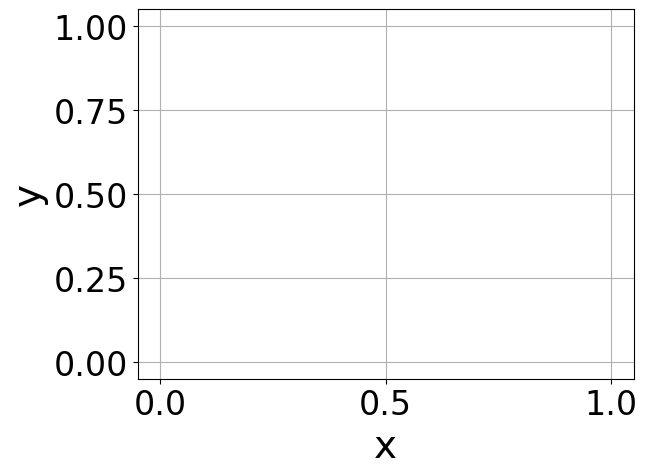
\includegraphics[width=0.5\textwidth]{../Figures/MA_8_F_1_2_graphR.png}
\end{center}
\begin{enumerate}[label=\Alph*.]
\item Yes, the graph is linear
\item No, the graph is not linear.

\end{enumerate} }
\litem{
Is the following relation a function?\[ (1, 4), (2, 16), (3, 36), (4, 64), (5, 64), (4, -4), (3, -16) \]\begin{enumerate}[label=\Alph*.]
\item Yes
\item No

\end{enumerate} }
\litem{
Is the equation below a linear function?\[ f(x) = -5(x + 1)+3 \]\begin{enumerate}[label=\Alph*.]
\item Yes, the equation is linear
\item No, the equation is not linear.

\end{enumerate} }
\litem{
Is the following relation a linear function?

\begin{tabular}{c|c}
x &y\tabularnewline \hline
-1 &-5\tabularnewline \hline
0 &1\tabularnewline \hline
1 &7\tabularnewline \hline
2 &13\tabularnewline \hline
3 &19\tabularnewline \hline
4 &25\tabularnewline \hline
5 &31\end{tabular}\begin{enumerate}[label=\Alph*.]
\item Yes
\item No

\end{enumerate} }
\end{enumerate}

\end{document}